\documentclass[12pt]{article}
\usepackage[english]{babel}
\usepackage[english]{isodate}
\usepackage[table,svgnames]{xcolor}
\usepackage{url}
\usepackage[utf8x]{inputenc}
\usepackage[T1]{fontenc}
\usepackage{longtable}
\usepackage{amsmath}
\usepackage{graphicx}
\usepackage{parskip}
\usepackage{fancyhdr}
\usepackage{vmargin}
\usepackage{hyperref}
\usepackage{pgfgantt}
\usepackage{pgf-umlcd}
\usepackage{xparse}
\usepackage{float}
\usepackage{tabularx}
\usepackage{titling}
\usepackage{fancyhdr}
\usepackage{rotating}
\usepackage{lscape}
\usepackage[landscape]{geometry}


% Global graphiscspath
\graphicspath{{../../../img/}}

% Styling changes

%% Better margins
%\setmarginsrb{1 cm}{1 cm}{1 cm}{1 cm}{0 cm}{0 cm}{0 cm}{0 cm}


\begin{document}
\pagestyle{empty}

  \begin{figure}[ht]

  	\begin{center}
  	
  	
  	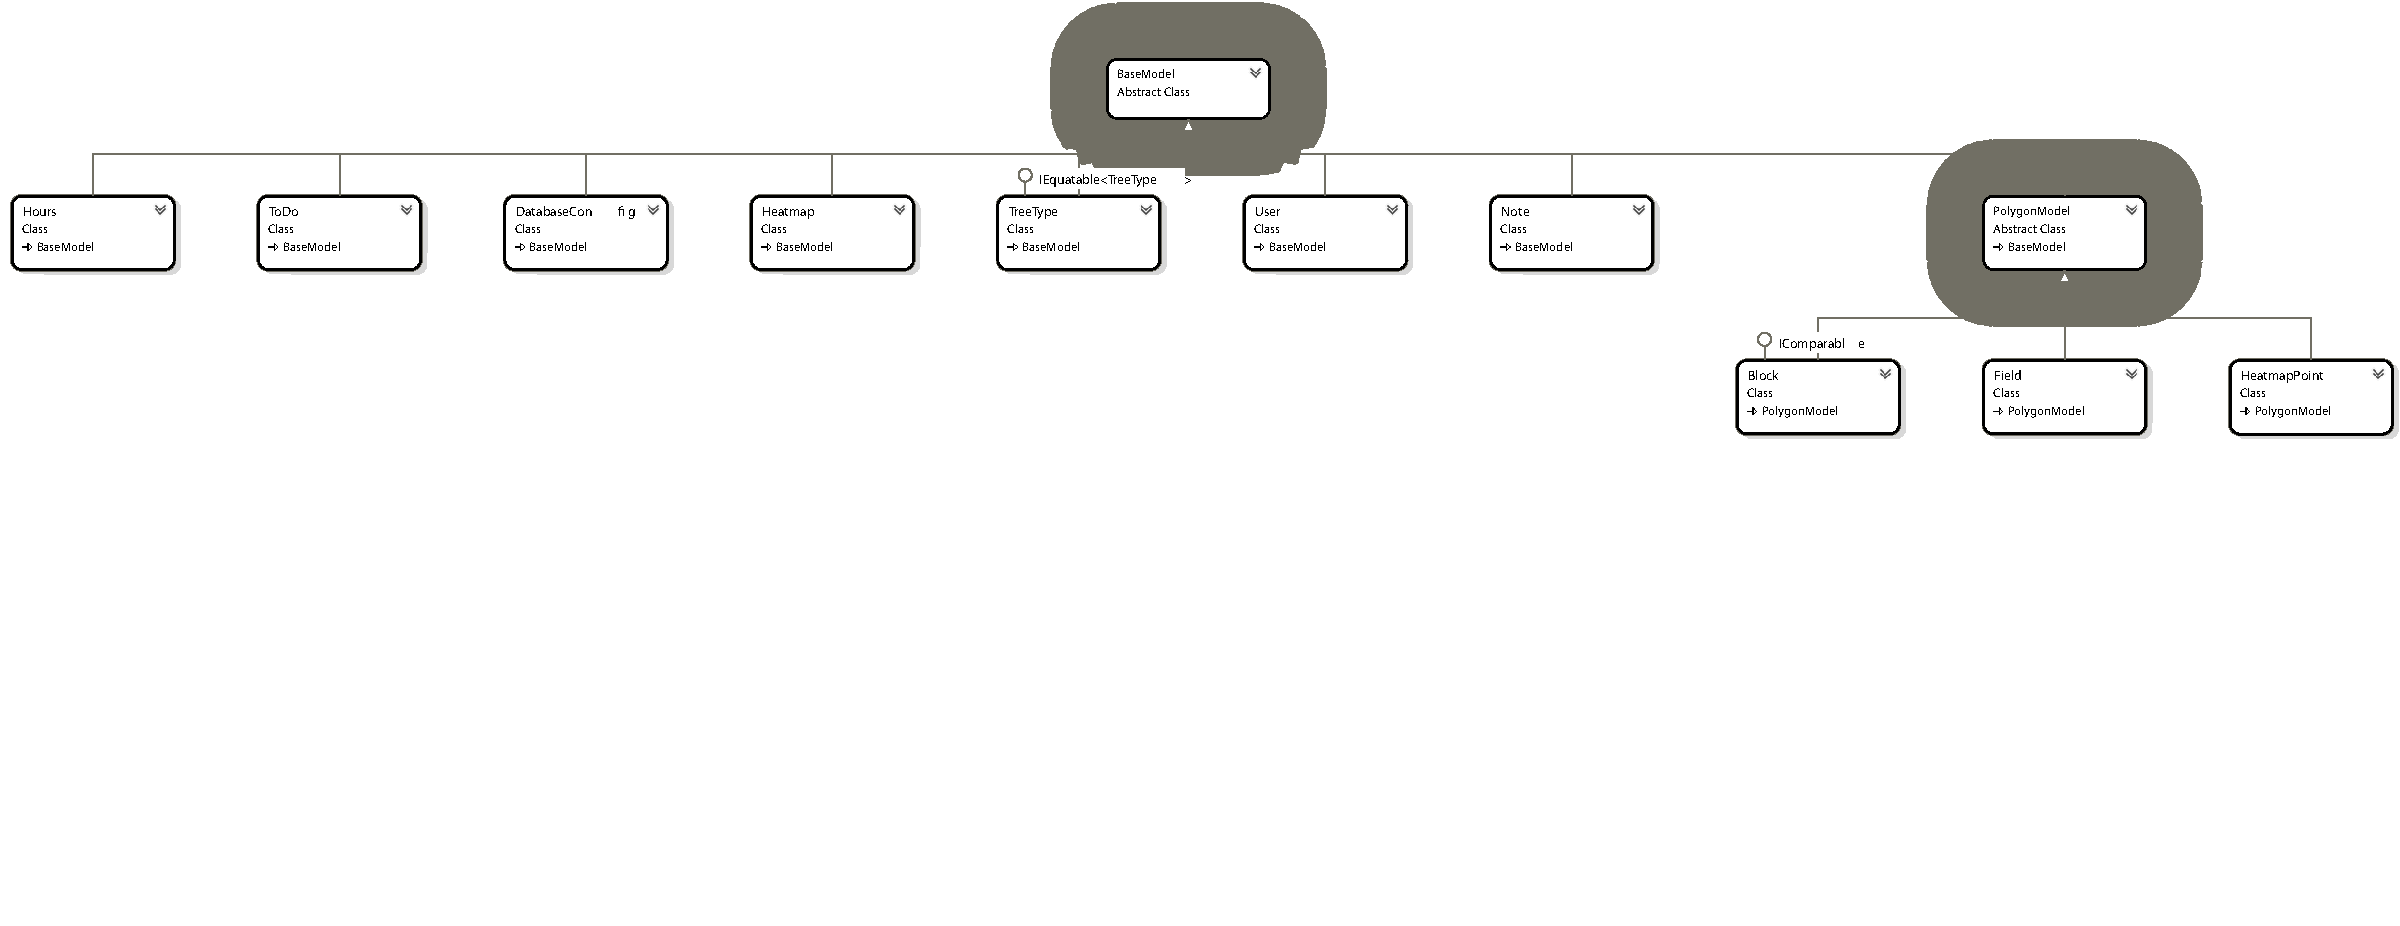
\includegraphics[width=0.9\paperwidth, keepaspectratio=true]{ClassDiagram1-part1.pdf}
  	\caption{Classdiagramm forms part1}\label{classdiagram}\
  	\end{center}
  \end{figure}


  \begin{figure}[ht]

  	\centering
  	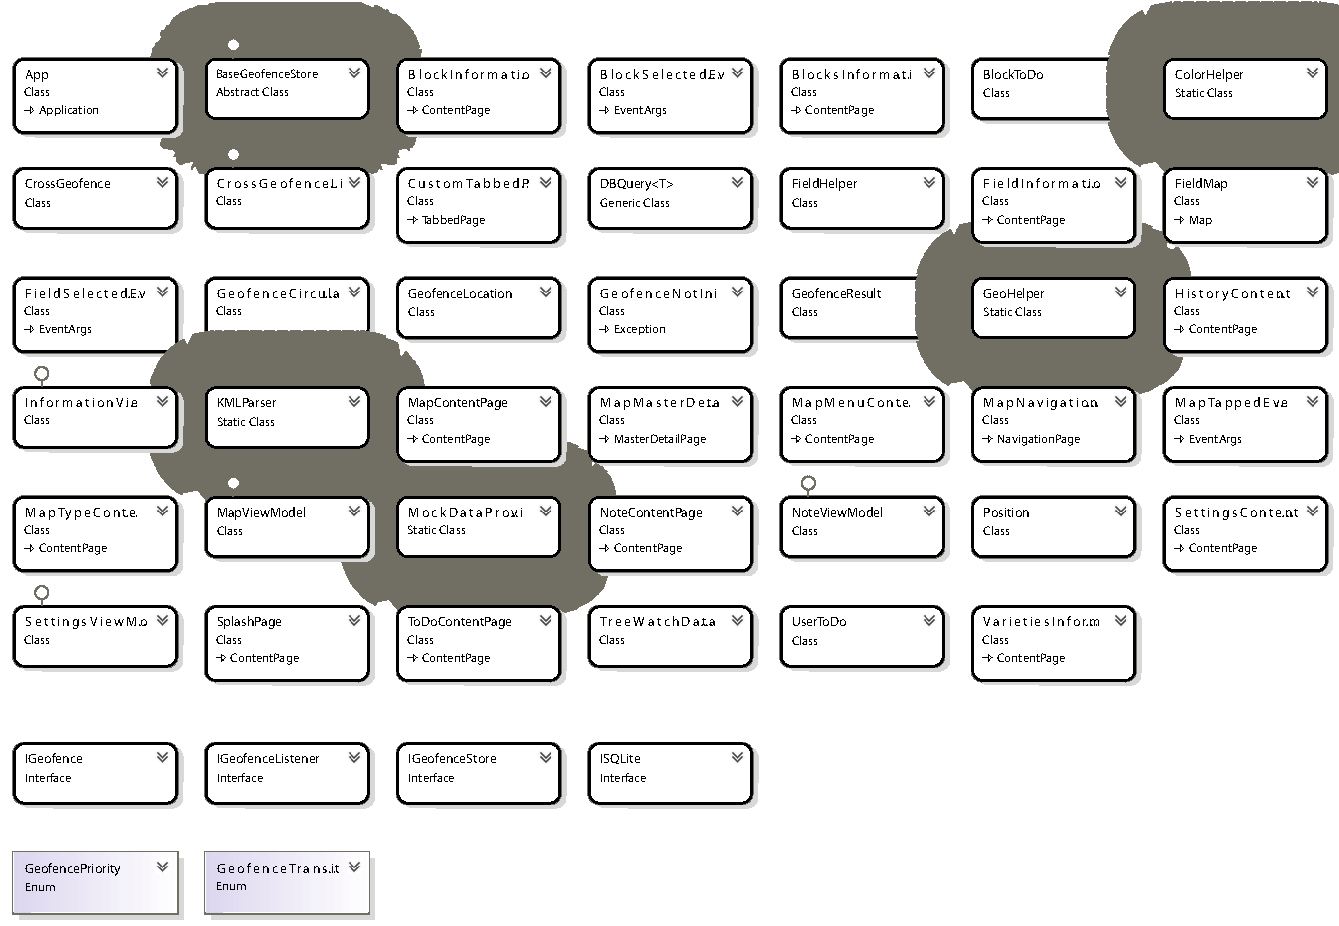
\includegraphics[width=0.9\paperwidth, keepaspectratio=true]{ClassDiagram1-part2.pdf}
  	\caption{Classdiagramm forms part2}\label{classdiagram}\
  \end{figure}
  
  \clearpage

  \begin{figure}[ht]

  	\centering
  	
\includegraphics[width=0.9\paperwidth, keepaspectratio=true]{ClassDiagramiOS.pdf}
  	\caption{Classdiagramm ios}\label{classdiagram}\
  \end{figure}

  \begin{figure}[ht]

  	\centering
  	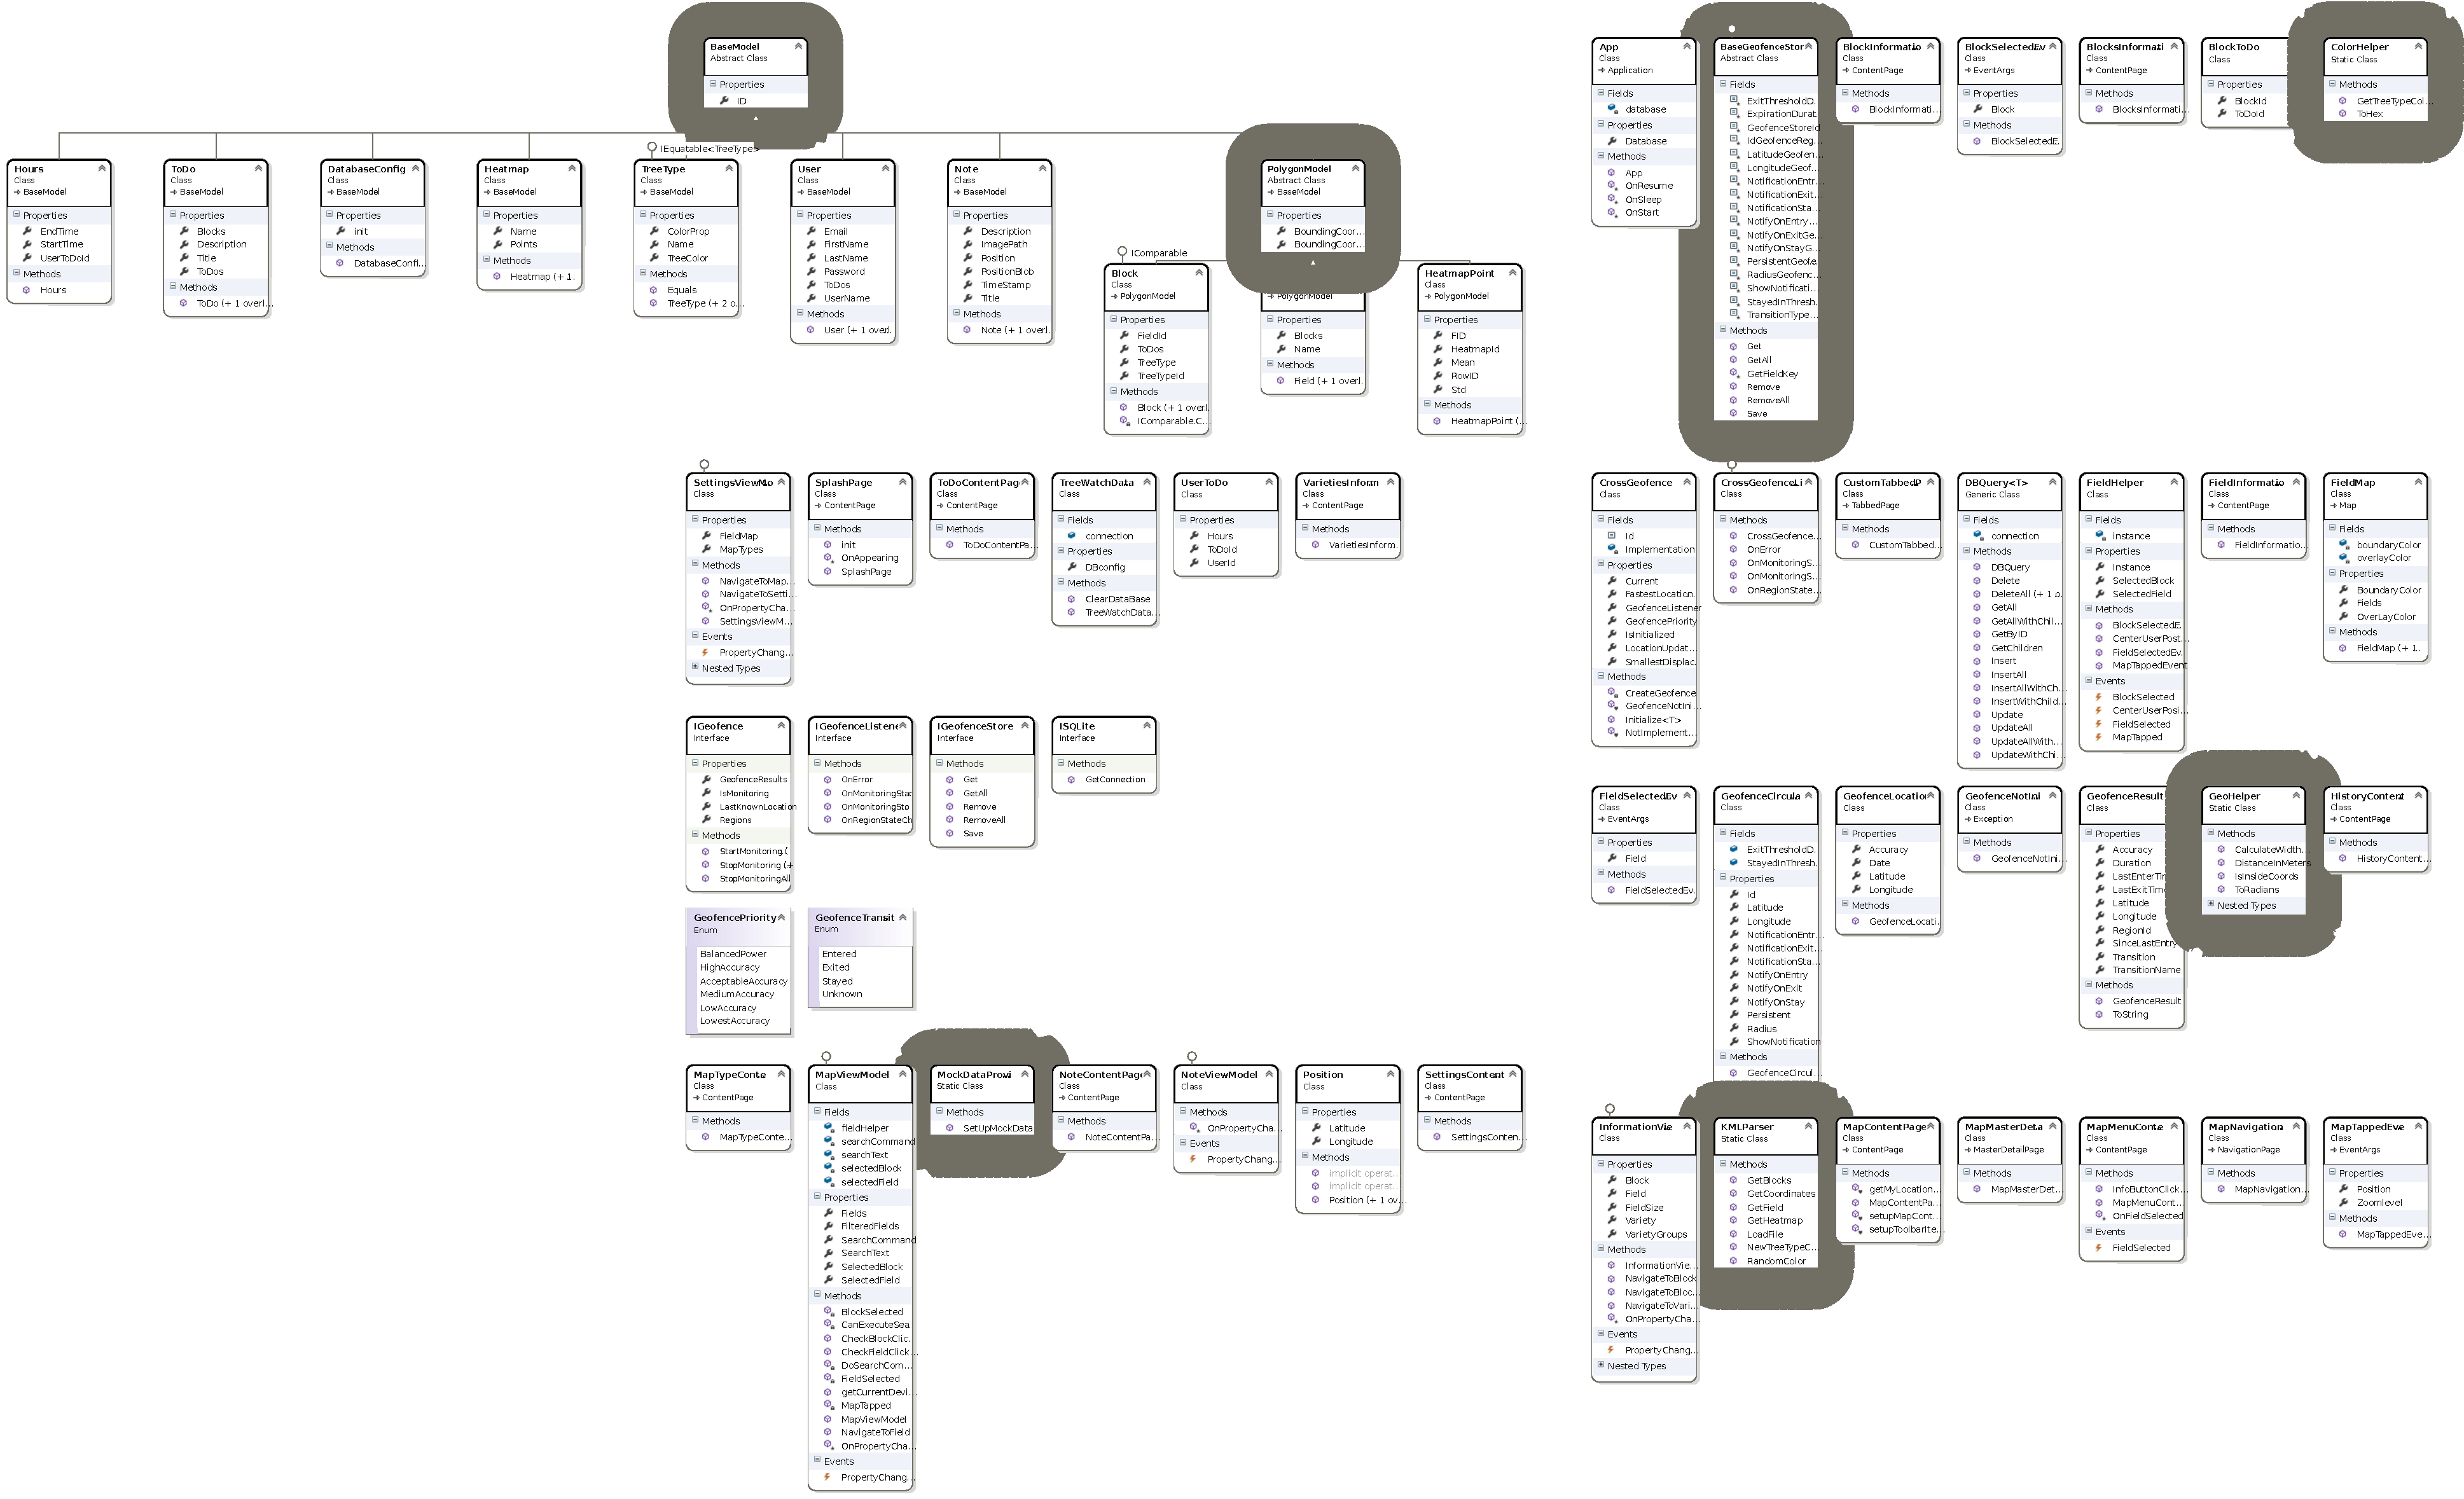
\includegraphics[width=0.9\paperwidth, keepaspectratio=true]{ClassDiagramForms.pdf}
  	\caption{Classdiagramm Forms}\label{classdiagram}\
  \end{figure}

\end{document}
